%!TEX root = ../thesis.tex

\chapter{Протоколи IPSec}
\label{chap:review}  %% відмічайте кожен розділ певною міткою -- на неї наприкінці необхідно посилатись

\section{Особливості реалізації криптографічних механізмів протоколів IPSec}

IPSec (Internet Protocol Security) є набором протоколів для забезпечення захисту передачі даних в IP-мережах. Його криптографічні механізми ґрунтуються на шифруванні, автентифікації, цілісності даних та управлінні ключами. Основні протоколи, що складають IPSec, включають Authentication Header (AH) та Encapsulating Security Payload (ESP), а також механізм Internet Key Exchange (IKE) для обміну ключами.

\subsection{Authentication Header (AH)}

AH забезпечує автентифікацію джерела даних та гарантує цілісність IP-пакетів, захищаючи їх від модифікацій під час передачі. Цей протокол додає до пакета спеціальний заголовок, який містить криптографічний хеш (наприклад, HMAC-SHA1 або HMAC-SHA256), розрахований з урахуванням певного секретного ключа. Формула для хешування виглядає так:
$$HMAC = H\left(K \oplus opad || H\left(K \oplus ipad || Message\right)\right),$$
де $K$ – це секретний ключ, а $ipad$ та $opad$ – константи для внутрішнього та зовнішнього заповнення.

AH застосовується до IP-заголовка і, зазвичай, не шифрує дані, але забезпечує їхню цілісність і аутентифікацію. Його головний недолік — відсутність конфіденційності, що означає, що дані залишаються видимими для третіх сторін.

\subsection{Encapsulating Security Payload (ESP)}

ESP реалізує шифрування, а також автентифікацію даних, що забезпечує конфіденційність, цілісність і автентичність повідомлень. У транспортному режимі ESP шифрує лише корисні дані (payload), а в тунельному режимі — весь IP-пакет, включаючи заголовок. Основні алгоритми шифрування для ESP — AES і 3DES. Формула для шифрування пакету:
$$C = Encrypt_{AES}(K, Payload),$$
де $C$ — зашифроване повідомлення, $K$ — секретний ключ, а $Payload$ — дані пакету.

У тунельному режимі ESP створює додатковий IP-заголовок, щоб захистити оригінальну IP-адресу від перехоплення, що є важливим для захисту внутрішньої мережі організації від атак.

\subsection{Internet Key Exchange (IKE)}

IKE відповідає за обмін ключами і встановлення Security Association (SA) — набору параметрів безпеки, що визначають тип захисту для з'єднання. Основним механізмом IKE є протокол Diffie-Hellman для встановлення загальних ключів, що використовуються для шифрування та автентифікації. Формула обміну:
$$K_{AB} = g^{a \cdot b} \mod p,$$
де $a$ та $b$ — секретні ключі сторін, а $g$ та $p$ — спільні параметри.

IKE використовує два порти (500 та 4500) для підтримки NAT-Traversal, що забезпечує сумісність з мережами, де змінюються IP-адреси під час пересилання пакетів через маршрутизатори, що використовують NAT.

\section{Основне призначення протоколів IPSec та взаємодія зі стеком протоколів TCP/IP}

Протоколи IPSec (Internet Protocol Security) використовуються для захисту передачі даних на мережевому рівні (Layer 3) моделі OSI. Вони забезпечують цілісність, автентифікацію та конфіденційність даних шляхом шифрування та контролю автентичності IP-пакетів. Основною перевагою IPSec є його незалежність від додатків, оскільки він працює на рівні IP. Це дозволяє захищати всі протоколи вищих рівнів (таких як TCP і UDP) та мережеві додатки, незалежно від їхнього типу.

На відміну від інших протоколів безпеки, таких як TLS (Transport Layer Security), що працює на транспортному рівні (Layer 4), або SSH (Secure Shell), який функціонує на прикладному рівні (Layer 7), IPSec забезпечує безпеку безпосередньо на рівні IP-пакетів. Завдяки цьому він може захищати будь-який тип даних, що передається через IP, забезпечуючи універсальну конфіденційність і цілісність трафіку на основі IP.

Взаємодія IPSec із протоколами стеку TCP/IP реалізується через його ключові компоненти — Authentication Header (AH) та Encapsulating Security Payload (ESP).

У контексті стеку TCP/IP IPSec автоматично забезпечує захист мережевого рівня (Internet Layer), дозволяючи захищати всі транспортні протоколи (TCP, UDP) та додатки, які їх використовують. Це робить IPSec універсальним рішенням для забезпечення безпеки корпоративних мереж, зокрема для реалізації VPN-з'єднань. Таким чином, IPSec гарантує безпечну передачу даних між віддаленими мережами та пристроями, забезпечуючи захист як у межах локальних мереж, так і при використанні глобального Інтернету.

\section{Архітектура стеку протоколів IPSec}

Архітектура стеку протоколів IPSec представлена у вигляді багаторівневої структури, яка забезпечує комплексний підхід до безпеки IP-мереж. IPSec складається з ряду протоколів, механізмів та алгоритмів, які взаємодіють між собою для забезпечення конфіденційності, цілісності та автентифікації даних на мережевому рівні.

\begin{figure}[h!]
    \centering
    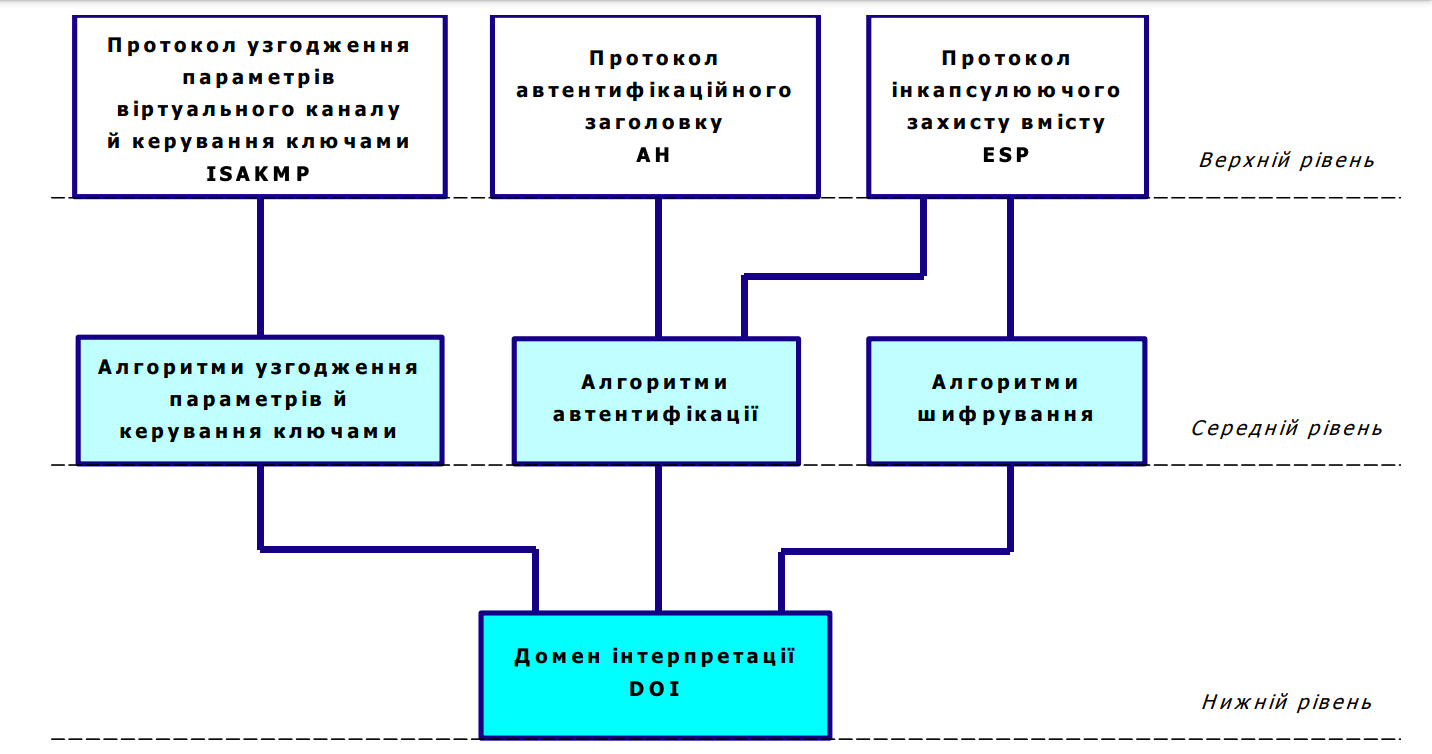
\includegraphics[scale=0.33]{IMAGES/IPSec_architecture.png}
    \caption{Архітектура стеку протоколів IPSec.}
    \label{fig_ipsec_architecture}
\end{figure}

На верхньому рівні архітектури IPSec зосереджені ключові протоколи та механізми, які забезпечують основні функції безпеки:
\begin{itemize}
    \item \textbf{Authentication Header (AH)} — забезпечує автентифікацію джерела даних і контроль цілісності IP-пакетів, проте не забезпечує конфіденційності.
    \item \textbf{Encapsulating Security Payload (ESP)} — відповідає за шифрування, автентифікацію та цілісність даних, забезпечуючи конфіденційність переданої інформації.
    \item \textbf{Internet Security Association and Key Management Protocol (ISAKMP)} — регламентує встановлення та управління безпечними асоціаціями (SA), а також координує узгодження параметрів безпеки.
\end{itemize}

Середній рівень архітектури включає механізми та алгоритми для:
\begin{itemize}
    \item узгодження параметрів шифрування та автентифікації;
    \item вибору криптографічних алгоритмів відповідно до вимог безпеки (наприклад, AES, HMAC-SHA-256 тощо);
    \item реалізації протоколів обміну ключами, таких як IKE (Internet Key Exchange) і його вдосконалена версія IKEv2.
\end{itemize}

Нижній рівень архітектури забезпечує підтримку інтероперабельності через використання \textbf{Domain of Interpretation (DOI)}. DOI виконує роль стандарту, який визначає набір параметрів і правил для взаємодії між різними реалізаціями IPSec, включаючи ідентифікатори криптографічних алгоритмів, параметри політик безпеки та формати даних.

\subsection{Режими передачі в IPSec}
IPSec підтримує два основних режими передачі:

\begin{enumerate}
    \item \textbf{Транспортний режим}: захищає лише корисне навантаження пакета, залишаючи IP-заголовок без змін. Використовується для прямого з’єднання між пристроями (host-to-host).

    \begin{figure}[h!]
        \centering
        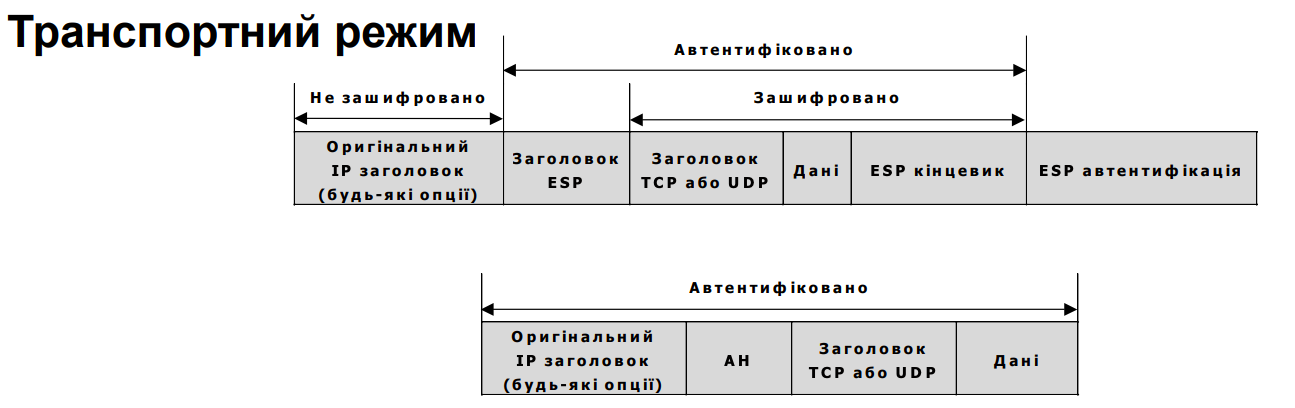
\includegraphics[scale=0.35]{IMAGES/transport_mode.png}
        \caption{Транспортний режим у IPSec.}
        \label{fig_transport_mode}
    \end{figure}
    
    \item \textbf{Тунельний режим}: захищає весь пакет, включаючи заголовок IP. Використовується для з’єднання між мережевими шлюзами (gateway-to-gateway).

    \begin{figure}[h!]
        \centering
        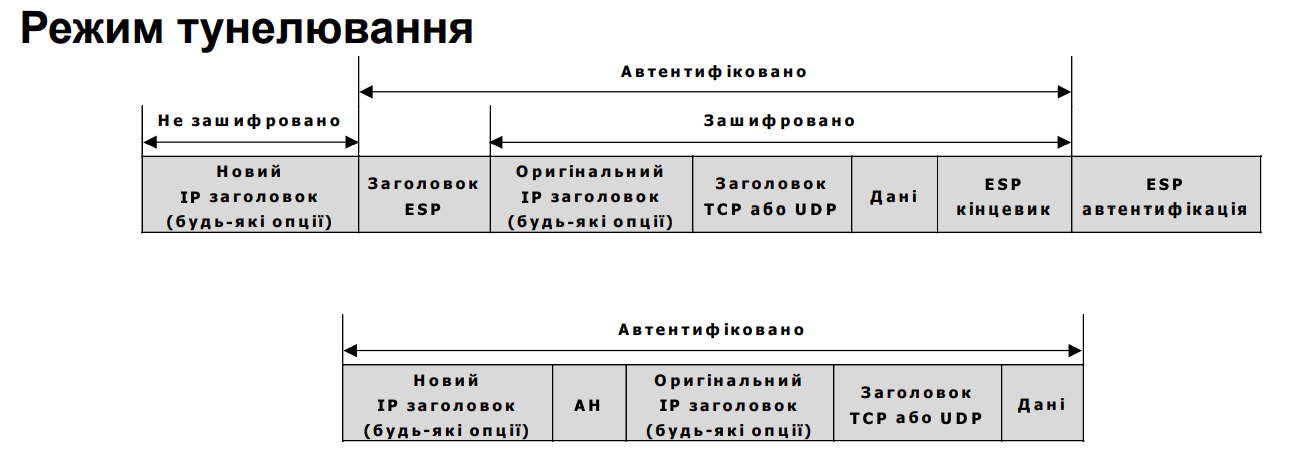
\includegraphics[scale=0.35]{IMAGES/tunnel_mode.png}
        \caption{Тунельний режим у IPSec.}
        \label{fig_tunnel_mode}
    \end{figure}

\end{enumerate}

\subsection{Основні принципи побудови архітектури}
Архітектура IPSec спроєктована таким чином, щоб забезпечити:
\begin{itemize}
    \item \textbf{Гнучкість:} підтримка різних сценаріїв використання (хост-хост, шлюз-шлюз, хост-шлюз).
    \item \textbf{Модульність:} можливість додавання нових криптографічних алгоритмів і протоколів без кардинальних змін у базовій структурі.
    \item \textbf{Інтеграція:} сумісність із стеком TCP/IP, що дозволяє захищати всі рівні транспортного протоколу (TCP, UDP) і додатки, які їх використовують.
\end{itemize}

\section{Призначення, особливості та відмінності криптографічних механізмів протоколів AH, ESP, ISAKMP, IKE, IKEv2, KINK та ін.}

Протоколи IPSec, такі як AH (Authentication Header), ESP (Encapsulating Security Payload), ISAKMP (Internet Security Association and Key Management Protocol), IKE (Internet Key Exchange), IKEv2, та KINK (Kerberized Internet Negotiation of Keys), використовуються для забезпечення безпеки, аутентифікації та конфіденційності в IP-мережах. Кожен із цих протоколів має своє особливе призначення та механізми роботи.

\subsection{AH (Authentication Header)}
Основна мета: Забезпечення аутентифікації джерела та цілісності даних IP-пакетів.
\par Особливості: AH використовує HMAC для автентифікації даних та не забезпечує шифрування (тобто, не гарантує конфіденційності).
\par Призначення: Відкрито захищає цілісність даних, зокрема, шляхом перевірки на справжність всього пакету, окрім змінних полів (наприклад, IP TTL).

\subsection{ESP (Encapsulating Security Payload)}
Основна мета: Забезпечення конфіденційності, аутентифікації та цілісності.
\par Особливості: ESP надає шифрування та цілісність даних за допомогою криптографічних методів (AES, 3DES). У деяких реалізаціях також додається підтримка аутентифікації.
\par Відмінність від AH: ESP захищає тільки корисне навантаження пакету (тобто, він забезпечує конфіденційність), але не аутентифікує IP заголовок.

\subsection{ISAKMP (Internet Security Association and Key Management Protocol)}
Основна мета: Створення, обробка та видалення Security Associations (SA), що відповідають за організацію захищених каналів зв’язку.
\par Особливості: ISAKMP забезпечує незалежну від протоколів IPsec роботу та може використовуватися для аутентифікації різними методами (наприклад, з використанням сертифікатів).
\par Переваги: ISAKMP не обмежується жодним конкретним криптоалгоритмом, а отже може бути оновлений для підтримки нових алгоритмів та протоколів (наприклад, IKE та IKEv2).

\subsection{IKE (Internet Key Exchange)}
Основна мета: Автентифікація та управління ключами.
\par Особливості: IKE об’єднує в собі ISAKMP, OAKLEY та SKEME, що дозволяє автоматизувати створення та захист каналів передачі. IKE працює в двох фазах — для встановлення SAs (Security Associations) та для забезпечення стійкого зв’язку.

\subsection{IKEv2}
Особливості: Відрізняється від IKE більш оптимізованими функціями управління ключами та покращеною стійкістю до збоїв.
\par Оновлення: IKEv2 використовує надійніші методи шифрування та автентифікації, зокрема алгоритми групового обміну ключами (Diffie-Hellman) та перевірки ідентичностей.

\subsection{KINK (Kerberized Internet Negotiation of Keys)}
Основна мета: Полегшення обміну ключами для IPsec, використовуючи автентифікацію за допомогою протоколу Kerberos.
\par Особливості: Цей протокол використовує наявну систему Kerberos для генерації ключів без необхідності вручну налаштовувати IPSec. Це полегшує конфігурацію в мережах, де використовується Kerberos для автентифікації користувачів.

\section{Концепція безпечних асоціацій (SA) та бази даних SPD і SAD}

\subsection{Концепція безпечних асоціацій (SA)}

У протоколах IPSec поняття безпечної асоціації (Security Associations, SA) є ключовим, оскільки воно визначає налаштування, за допомогою яких забезпечується безпека обміну даними між двома вузлами. SA встановлює, які методи автентифікації та шифрування застосовувати для певного каналу зв’язку. В IPSec кожна SA є унікальною для напрямку передачі: для кожної з двох сторін зв'язку встановлюється своя SA (тобто одна для передавання та одна для приймання даних). Кожна SA містить такі компоненти:

\begin{enumerate}
    \item Security Parameters Index (SPI) – унікальний ідентифікатор, який використовується для відстеження окремих SA в IPSec.
    \item Тип протоколу – AH (Authentication Header) або ESP (Encapsulating Security Payload).
    \item IP-адреса призначення – адреса кінцевої точки SA.
\end{enumerate}

SA зберігаються у базі даних безпечних асоціацій (Security Associations Database, SAD), яка надає контекст для обробки вхідних і вихідних пакетів згідно з параметрами захисту. Наприклад, коли пристрій IPSec отримує пакет, він шукає SPI в SAD, щоб визначити відповідну SA для автентифікації або шифрування даних пакета.

\subsection{База даних політик безпеки (SPD)}

База даних політик безпеки (Security Policy Database, SPD) містить правила, які визначають, як слід обробляти трафік відповідно до політики безпеки. SPD містить три основних дії для трафіку:

\begin{itemize}
    \item PROTECT: трафік захищається за допомогою шифрування або автентифікації відповідно до визначених у SA параметрів.
    \item BYPASS: трафік передається без захисту.
    \item DISCARD: трафік відхиляється.
\end{itemize}

SPD, таким чином, є "фільтром" для пакету даних, визначаючи, який трафік підлягає захисту, а який – ні. Якщо правило в SPD визначає, що трафік потребує захисту, він посилається на SAD для визначення конкретної SA, яка буде використана для цього трафіку.

\subsection{Взаємодія SPD і SAD}

\begin{enumerate}
    \item Коли пакет надходить у систему, IPSec перевіряє його відповідність до правил у SPD.
    \item Якщо трафік відповідає правилу "PROTECT", IPSec звертається до SAD, щоб знайти відповідну SA на основі SPI.
    \item Якщо SA у SAD не знайдено, система ініціює новий процес для встановлення безпечної асоціації, як правило, за допомогою протоколу IKE або IKEv2.
\end{enumerate}

Таким чином, SPD визначає, який трафік потребує захисту, а SAD надає параметри для цього захисту.

\section{Особливості структури заголовків протоколів AH і ESP в тунельному та транспортному режимах з повним описанням їх полів та можливих значень}

IPSec використовує два основні протоколи, Authentication Header (AH) та Encapsulating Security Payload (ESP), кожен з яких має специфічну структуру заголовків та режими роботи — тунельний та транспортний.

\subsection{Заголовок AH}

\begin{figure}[h!]
        \centering
        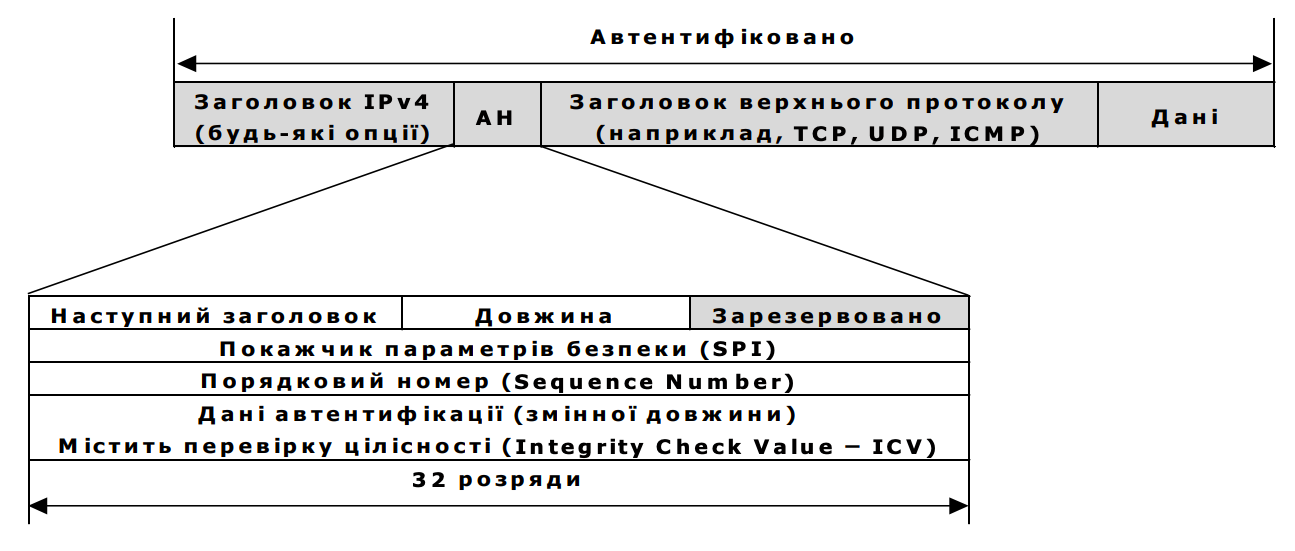
\includegraphics[scale=0.35]{IMAGES/AH_title.png}
        % \caption{Количество круговых диаграмм, похожих на Пэкмена}
        \label{fig_pacman}
\end{figure}

AH забезпечує автентифікацію джерела та цілісність даних IP-пакету без шифрування. Основні поля заголовка AH включають:

\begin{itemize}
    \item Next Header (8 біт): ідентифікує наступний протокол в пакеті.
    \item Payload Length (8 біт): вказує довжину заголовка AH.
    \item Reserved (16 біт): зарезервовано для майбутнього використання.
    \item Security Parameters Index (SPI) (32 біт): визначає асоціацію безпеки для пакету.
    \item Sequence Number (32 біт): захист від атак повтору (replay attacks).
    \item Integrity Check Value (ICV) (перемінна довжина): містить хеш для перевірки цілісності пакету.
\end{itemize}

У транспортному режимі AH додає свій заголовок між IP-заголовком та корисним навантаженням, а в тунельному режимі — на початку новоствореного зовнішнього IP-заголовка, забезпечуючи цілісність і автентифікацію всього внутрішнього IP-пакету. Це робить AH більш вразливим до змін у заголовках (наприклад, через NAT), що обмежує його використання в порівнянні з ESP.

\subsection{Заголовок ESP}

\begin{figure}[h!]
        \centering
        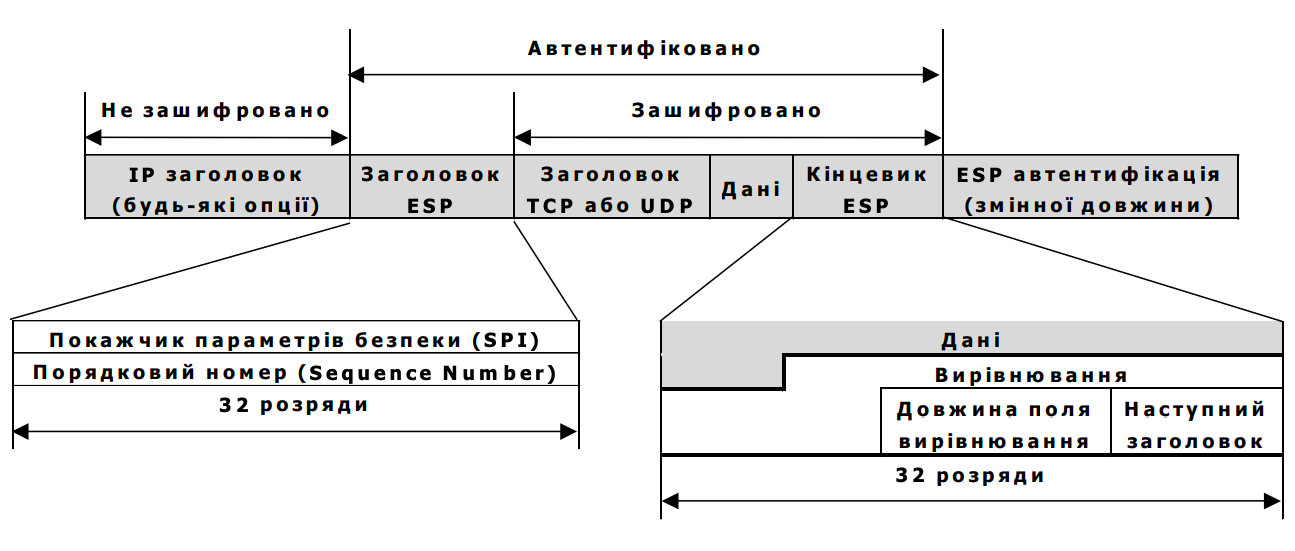
\includegraphics[scale=0.35]{IMAGES/ESP_protoc.png}
        % \caption{Количество круговых диаграмм, похожих на Пэкмена}
        \label{fig_pacman}
\end{figure}

ESP надає як автентифікацію, так і шифрування. Його структура складається з:

\begin{itemize}
    \item SPI (32 біт): визначає асоціацію безпеки для ESP.
    \item Sequence Number (32 біт): захист від атак повтору.
    \item Encrypted Payload: зашифрований корисний вантаж.
    \item ESP Trailer: містить інформацію про кінцевий маркер даних.
    \item ESP Authentication (опціонально): забезпечує автентифікацію даних.
\end{itemize}

У транспортному режимі ESP шифрує лише корисне навантаження IP-пакету, залишаючи оригінальний IP-заголовок відкритим. У тунельному режимі, натомість, шифрується весь внутрішній пакет разом із оригінальним IP-заголовком, а зовні додається новий IP-заголовок, що робить цей режим оптимальним для захищеного з’єднання між мережами через небезпечні середовища, наприклад, Інтернет.

\vspace{0.5cm}
\textbf{Порівняння AH і ESP}
\begin{table}[h!]
\centering
\begin{tabular}{|l|l|l|}
\hline
\rowcolor{gray!30} \textbf{Поле}             & \textbf{AH}                                      & \textbf{ESP}                                    \\ \hline
Шифрування          & \cellcolor{red!20}Ні                          & \cellcolor{green!20}Так                         \\ \hline
Автентифікація      & \cellcolor{green!20}Так                       & \cellcolor{gray!20}Опціонально                  \\ \hline
Захист від повторів & \cellcolor{green!20}Так                       & \cellcolor{green!20}Так                         \\ \hline
Режими              & \cellcolor{gray!20}Транспортний і тунельний   & \cellcolor{gray!20}Транспортний і тунельний     \\ \hline
Сумісність з NAT    & \cellcolor{red!20}Погано сумісний             & \cellcolor{green!20}Краще сумісний              \\ \hline
\end{tabular}
\caption{Порівняння AH і ESP}
\label{tab:comparison}
\end{table}

Таким чином, ESP є більш універсальним через підтримку шифрування, тоді як AH обмежений забезпеченням тільки цілісності та автентифікації без шифрування, що робить його менш захищеним у відкритих мережах.

\section{Особливості обробки вхідних та вихідних IPSec-пакетів для кожного з протоколів та режимів}

Процес обробки вхідних і вихідних пакетів у протоколах IPSec, таких як AH і ESP, залежить від режиму використання (транспортного чи тунельного) і типу пакета (вхідний або вихідний).

\textbf{Обробка вхідних пакетів}:
\begin{enumerate}
    \item AH у транспортному режимі:
    AH використовується для автентифікації даних. Після отримання пакета пристрій перевіряє автентичність заголовка та його цілісність, використовуючи алгоритми, визначені в заголовку AH.
    Поле заголовка AH включає значення хеш-функції (наприклад, HMAC), яке приймаюча сторона повинна перевірити, щоб переконатися, що дані не були змінені під час передачі.
    \item AH у тунельному режимі:
    Весь оригінальний IP-пакет вкладається у новий IP-заголовок і захищається AH. Усі внутрішні IP-дані перевіряються, що забезпечує цілісність і автентичність не тільки верхніх рівнів даних, але й оригінального IP-заголовка.
    \item ESP у транспортному режимі:
    У транспортному режимі ESP захищає лише дані транспортного рівня, залишаючи оригінальний IP-заголовок незахищеним. Після отримання пакета пристрій декриптує і перевіряє цілісність корисного навантаження.
    Поля для автентифікації можуть бути відсутні, якщо ESP використовується лише для шифрування.
    \item ESP у тунельному режимі:
    Усі дані оригінального пакета, включно з IP-заголовком, шифруються й автентифікуються. Після отримання пристрій видаляє зовнішній IP-заголовок, розшифровує та перевіряє дані, включаючи внутрішній заголовок.
\end{enumerate}

\textbf{Обробка вихідних пакетів}:
\begin{enumerate}
    \item AH у транспортному режимі:
    Після формування вихідного IP-пакета пристрій додає заголовок AH між IP-заголовком і корисним навантаженням. Виконується обчислення автентифікаційного значення, яке додається в заголовок AH для подальшої перевірки отримувачем.
    \item AH у тунельному режимі:
    Пристрій створює новий IP-заголовок, що інкапсулює весь оригінальний пакет, і додає AH між новим і оригінальним заголовками. Далі обчислюється значення автентифікації, яке підтверджує цілісність усього пакета.
    \item ESP у транспортному режимі:
    Перед відправкою дані пакетів шифруються, після чого додаються заголовок ESP і значення автентифікації (якщо застосовується). Таким чином, захищаються тільки дані транспортного рівня, а IP-заголовок залишається без змін.
    \item ESP у тунельному режимі:
    Весь оригінальний IP-пакет шифрується, включно з заголовком, і інкапсулюється у новий IP-заголовок. Цей режим забезпечує повний захист внутрішнього пакета і часто використовується для VPN-з’єднань.
\end{enumerate}

Такий підхід до обробки пакетів дозволяє адаптувати IPSec до різних сценаріїв захисту мережевого трафіку, від забезпечення цілісності даних до їхнього повного шифрування і захисту IP-інформації.

\section{Нижнiй рiвень архiтектури стеку протоколiв IPSec
– домен iнтерпретацiї DOI}

Домен інтерпретації (Domain of Interpretation, DOI) є ключовим компонентом архітектури IPSec, який визначає параметри та політики, необхідні для встановлення та управління безпечними з'єднаннями. DOI забезпечує узгодженість між різними реалізаціями протоколів, встановлюючи стандарти для обміну інформацією та управління безпекою.

\subsection{Роль DOI в архітектурі IPSec}

DOI визначає набір параметрів, політик та процедур, які використовуються під час встановлення та управління безпечними з'єднаннями в IPSec. Він забезпечує узгодженість між різними реалізаціями протоколів, встановлюючи стандарти для обміну інформацією та управління безпекою.

\textbf{Основні функції DOI}:
\begin{enumerate}
    \item Визначення параметрів безпеки: DOI встановлює, які алгоритми шифрування та хешування можуть використовуватися, а також їхні параметри.
    \item Узгодження політик: DOI забезпечує, щоб обидві сторони з'єднання мали спільне розуміння політик безпеки, що застосовуються.
    \item Ідентифікація протоколів: DOI визначає, які протоколи та механізми використовуються для встановлення та управління безпечними з'єднаннями.
\end{enumerate}

\textbf{Структура DOI}:
\begin{itemize}
    \item Ідентифікатор DOI: унікальний номер, який визначає конкретний домен інтерпретації.
    \item Атрибути безпеки: набір параметрів, що визначають політики та алгоритми безпеки.
    \item Протоколи управління: механізми, що використовуються для обміну інформацією та управління безпекою.
\end{itemize}

\subsection{Взаємодія DOI з іншими компонентами IPSec}

DOI тісно інтегрований з іншими компонентами IPSec, такими як ISAKMP (Internet Security Association and Key Management Protocol). ISAKMP забезпечує загальну структуру для встановлення та управління асоціаціями безпеки, тоді як DOI визначає специфічні параметри та політики для цих асоціацій.

Домен інтерпретації (DOI) є невід'ємною частиною архітектури IPSec, яка забезпечує узгодженість та стандартизацію параметрів безпеки між різними реалізаціями протоколів. Він визначає, які алгоритми та політики можуть використовуватися, забезпечуючи надійне та безпечне з'єднання між сторонами.

\section{Зареєстрованi алгоритми автентифiкацiї, шифрування, геш-функцiй та ін. для IPSec}

IPSec (Internet Protocol Security) використовує різноманітні криптографічні алгоритми для забезпечення конфіденційності, цілісності та автентифікації даних під час їх передачі через мережу.

\subsection{Алгоритми шифрування}

\begin{itemize}
    \item Алгоритми шифрування забезпечують конфіденційність даних, перетворюючи їх у форму, недоступну для несанкціонованого доступу.
    \item DES (Data Encryption Standard): Симетричний блоковий шифр з довжиною ключа 56 біт. Через низьку стійкість до сучасних атак вважається застарілим.
    \item 3DES (Triple DES): Розширена версія DES, яка застосовує алгоритм тричі з різними ключами, забезпечуючи підвищену безпеку.
    \item AES (Advanced Encryption Standard): Симетричний блоковий шифр з довжиною ключа 128, 192 або 256 біт. Є стандартом для сучасних систем шифрування завдяки високій безпеці та ефективності.
    \item Blowfish: Симетричний блоковий шифр з довжиною ключа від 32 до 448 біт. Відомий своєю швидкістю та гнучкістю.
\end{itemize}

\subsection{Алгоритми автентифікації}

Алгоритми автентифікації гарантують, що дані надходять від достовірного джерела та не були змінені під час передачі.

\begin{itemize}
    \item HMAC-MD5 (Hashed Message Authentication Code with MD5): Використовує хеш-функцію MD5 для створення коду автентифікації повідомлення. Через виявлені вразливості MD5 рекомендується використовувати більш надійні альтернативи.

    \item HMAC-SHA-1: Застосовує хеш-функцію SHA-1 для генерації коду автентифікації. Хоча SHA-1 вважається більш безпечним, ніж MD5, існують рекомендації переходити на більш стійкі алгоритми.

    \item HMAC-SHA-256/384/512: Використовують хеш-функції сімейства SHA-2 з різною довжиною вихідного хешу, забезпечуючи вищий рівень безпеки.
\end{itemize}

\subsection{Хеш-функції}

Хеш-функції перетворюють вхідні дані довільної довжини у фіксований розмір, що використовується для перевірки цілісності даних.

\begin{itemize}
    \item MD5 (Message Digest Algorithm 5): Генерує 128-бітний хеш. Через виявлені криптографічні вразливості не рекомендується для використання в сучасних системах безпеки.
    \item SHA-1 (Secure Hash Algorithm 1): Генерує 160-бітний хеш. Хоча більш безпечний, ніж MD5, також має відомі вразливості.
    \item SHA-2 (SHA-256, SHA-384, SHA-512): Сімейство хеш-функцій, що генерують хеші довжиною 256, 384 та 512 біт відповідно. Рекомендуються для використання завдяки високій стійкості до атак.
\end{itemize}

\subsection{Алгоритми обміну ключами}

Для безпечного обміну ключами в IPSec використовуються наступні алгоритми:

DH (Diffie-Hellman): Протокол, що дозволяє двом сторонам безпечно обмінюватися криптографічними ключами через незахищений канал. Існують різні групи DH з різним рівнем безпеки (групи 1, 2, 5 тощо).

\subsection{Протоколи управління ключами}

IPSec використовує протоколи для узгодження параметрів безпеки та управління ключами:

IKE (Internet Key Exchange): Протокол для встановлення асоціацій безпеки та обміну ключами між двома сторонами. Існують версії IKEv1 та IKEv2, де IKEv2 пропонує покращену безпеку та ефективність.

Вибір конкретних алгоритмів залежить від вимог до безпеки та сумісності між сторонами з'єднання. Рекомендується використовувати сучасні та стійкі до відомих атак алгоритми, такі як AES для шифрування та HMAC-SHA-256 для автентифікації.

\section{Особливостi основних схем застосування протоколiв IPSec: хост-хост, шлюз-шлюз та хост-шлюз. А також використання протоколiв IPSec для побудови VPN-тунелiв}

IPSec (Internet Protocol Security) — це набір протоколів, що забезпечують захист даних на мережевому рівні шляхом шифрування та автентифікації IP-пакетів. Існують три основні схеми застосування IPSec: «хост-хост», «шлюз-шлюз» та «хост-шлюз». Крім того, IPSec широко використовується для побудови VPN-тунелів.

\subsection{Особливості основних схем застосування протоколів IPSec}
\begin{enumerate}
    \item Схема «хост-хост»
        \begin{figure}[h!]
            \centering
            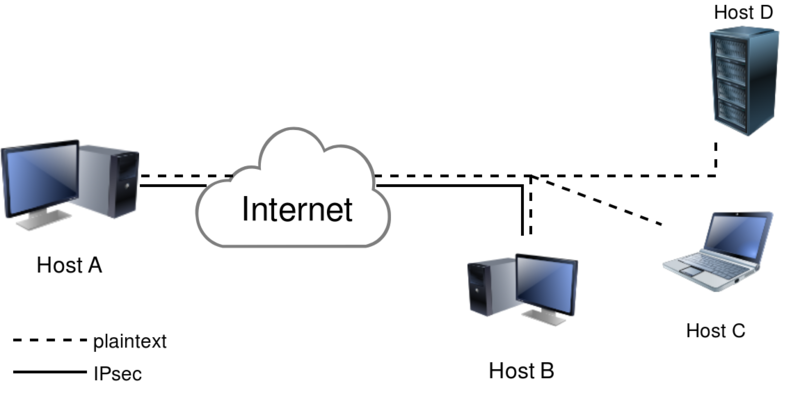
\includegraphics[scale=0.45]{IMAGES/host-to-host.png}
            % \caption{Количество круговых диаграмм, похожих на Пэкмена}
            \label{fig_pacman}
        \end{figure}
    \par У цій схемі захищене з'єднання встановлюється безпосередньо між двома кінцевими пристроями (хостами). Зазвичай використовується транспортний режим IPSec, який забезпечує шифрування та автентифікацію лише корисного навантаження IP-пакета, залишаючи заголовок без змін. Це підходить для захисту трафіку між двома конкретними пристроями в мережі.
    
    \item Схема «шлюз-шлюз»
        \begin{figure}[h!]
            \centering
            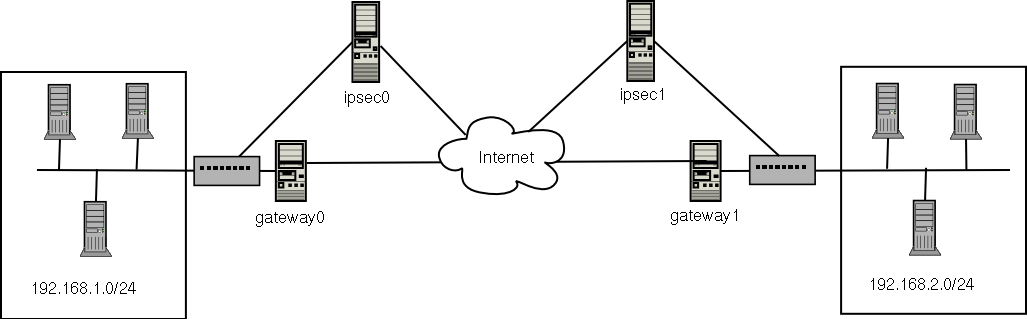
\includegraphics[scale=0.45]{IMAGES/net-to-net.png}
            % \caption{Количество круговых диаграмм, похожих на Пэкмена}
            \label{fig_pacman}
        \end{figure}
    \par У цій конфігурації захищене з'єднання встановлюється між двома мережевими шлюзами (наприклад, маршрутизаторами або брандмауерами), які з'єднують різні локальні мережі. Використовується тунельний режим IPSec, при якому весь IP-пакет (включаючи заголовок) інкапсулюється в новий IP-пакет з новим заголовком. Це дозволяє забезпечити захист даних між двома мережами через незахищене середовище, наприклад, Інтернет.

    \item Схема «хост-шлюз»
    \par У цій схемі один кінець з'єднання є кінцевим пристроєм (хостом), а інший — мережевим шлюзом. Це корисно для віддалених користувачів, які підключаються до корпоративної мережі через захищене з'єднання. Зазвичай використовується тунельний режим IPSec, що забезпечує безпечний доступ віддаленого хоста до ресурсів мережі через шлюз.
\end{enumerate}

\subsection{Використання IPSec для побудови VPN-тунелів}

IPSec широко застосовується для створення віртуальних приватних мереж (VPN), забезпечуючи захищений канал зв'язку через незахищені мережі, такі як Інтернет. VPN-тунелі на базі IPSec використовують тунельний режим для інкапсуляції та шифрування всього IP-пакета, що гарантує конфіденційність, цілісність та автентифікацію переданих даних.